\documentclass{beamer}
\let\Tiny=\tiny % Gets rid of font warning.
\usepackage{lmodern,amsmath,amssymb,listings}
\usepackage{spot}
\usepackage{fancybox}
\usepackage[skins,listings]{tcolorbox}
\tcbset{enhanced}
\usepackage{fancyvrb}
\usepackage[latin1]{inputenc}
\usepackage[T1]{fontenc}
\usetheme{Warsaw}
\setbeamertemplate{navigation symbols}{} % turn off slide navigation buttons at the bottom

\title[Implementing WGFEM]{Implementing the Weak Galerkin F.E.M.}
\subtitle{With a Focus on Generality}

\author{Stephen Harris \\ \texttt{scharris@ualr.edu}}
\date{Nov. 7, 2013}


\begin{document}

\begin{frame}
  \titlepage
\end{frame}

\begin{frame}
  \frametitle{Outline}
  \tableofcontents[pausesections]
\end{frame}

\section{Generality Goal}
\subsection{Generality Defined}

\begin{frame}
  \frametitle{What is Meant by Generality Here?}
  \pause
  The ability to most easily solve the widest variety of problems
    \begin{align*}
      \spot<7>{\mathfrak{a}}(u_h,v) & = (\spot<4>{f},v)\quad\quad\quad \forall{v} \in \spot<6>{V_{h0}} \\
      u_h & = \spot<4>{g} \text{ on } \partial\spot<5>{\Omega}
    \end{align*}
    for solution $u_h$ in piecewise polynomial approximation space $V_h$ on mesh \spot<5>{$M_h$} of \spot<5>{$\Omega$}.
  \pause

  \begin{block}{Method Should Allow ``Mix and Match'' of Parts}
    Should allow the ``actors'' above to easily be varied independently:
    \pause
    \begin{enumerate}[<+->]
      \item functions $f$ and $g$
      \item mesh $M_h$ on which $V_h$ members are piecewise polynomial
      \item approximation space, by choice of \emph{degree constraints} on polynomial pieces of $V_h$ members -- by monomial degree or maximum variable degree
      \item bilinear form $\mathfrak{a}: V_h \times V_h \rightarrow \mathbb{R}$
    \end{enumerate}
  \end{block}

\end{frame}

\begin{frame}
  \frametitle{How General is the Implementation?}
  \pause
  \begin{itemize}[<+->]
    \item Many problems solvable without code additions or changes.
      \begin{itemize}[<+->]
        \item Allow arbitrary functions for $f$ and $g$.
        \item Provided Meshes
          \begin{itemize}
            \item Triangle meshes from mesh generator (Gmsh).
            \item Rectangle meshes for any number of space dimensions.
          \end{itemize}
        \item Basis -- Support arbitrary \emph{degree constraints} for approximating polynomials on interiors and sides separately,
          using either monomial or variable degree.
        \item Laplace bilinear form provided. 
      \end{itemize}
    \item Extensible in areas expected to frequently need changes.
      \begin{itemize}
        \item New problems solved by plugging in new code at \emph{plugin points}.
        \item Major plugin points are provided for
          \begin{itemize}
            \item variational bilinear form, $\mathfrak{a}$
            \item mesh -- Arbitrary polytope meshes for any space dimension can be supported. No uniformity requirements.
          \end{itemize}
        \item No mesh or vbf is ``built in'': provided ones use plugin system.
        \item Only \emph{new} aspects have to be coded for, thought about, and tested. Core method does not change.
      \end{itemize}
  \end{itemize}
\end{frame}

\subsection{The Means -- Abstraction and Modularity}

\subsubsection{Components: Limited Roles, Limited Knowledge}

\begin{frame}
  \frametitle{How? Components: Limited Roles, Limited Knowledge}
  Divide system into components having clear, limited roles.
  \pause
  \tcbset{left=1mm,right=1mm,bottom=1mm,top=1mm}
  \tcbox{Limited Role} \raisebox{3mm}{$\implies$} \raisebox{-0.2mm}{\tcbox{Limited Knowledge}}\\
  A component having a limited role means it also should have no knowledge of other components' internal workings.\\
  \pause
  Components should only depend on exposed operations of other components and their \emph{documented} behavior (usually the names).\\
  \pause
  Keep connections between components at a minimum!
  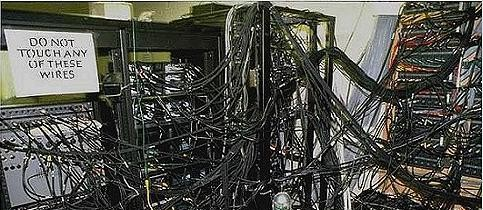
\includegraphics[height=3.5cm]{crazy-wiring.jpg}
\end{frame}

\subsubsection{Components for the WG Method}

\begin{frame}
  \frametitle{How Generality is Achieved: Abstraction and Modularity}
  Divide system into components having clear, limited roles.\\
  \pause
  \tcbset{colback =red!5!white, colframe =red!75!black, left=0mm,right=0mm,bottom=0mm,top=0mm}
  \begin{block}{Major Components}
    \tcbox{\shadowbox{Mesh}}
    \raisebox{1.4mm}{\shadowbox{WGrad Solver}}
    \raisebox{1.4mm}{\shadowbox{Basis}}
    \raisebox{1.25mm}{\shadowbox{Proj}}
    \tcbox{\shadowbox{VBF}}
    \raisebox{3.4mm}{\fbox{WG Solver}}
  \end{block}
  \pause
  \begin{block}{Auxiliary Types \& Components}
    \shadowbox{Monomial}
    \shadowbox{Polynomial}
    \shadowbox{Vector Monomial}
    \shadowbox{Weak Grad}
    \shadowbox{WG Solution}
    \raisebox{2mm}{\fbox{Error Norms}}
    \raisebox{2mm}{\fbox{Quadrature}}
    \raisebox{2mm}{\fbox{Linear Algebra}}
  \end{block}
  \pause
  \raisebox{-2mm}{\shadowbox{Shadowed}} components represent \emph{types}, with custom ops.
  \pause
  \raisebox{-2mm}{\tcbox{Enclosed}} types represent abstract
  types, or \emph{contracts}, as a set of operations which actual ``plugged in'' types must implement.
\end{frame}

\subsection{Bringing Components Together - Example}

\begin{frame}[fragile]{Bringing Components Together -- Example Run}
  \tcbset{colback =red!5!white, colframe =red!75!black, left=0mm,right=0mm,bottom=0mm,top=0mm, tcbox raise base}
  \begin{Verbatim}[gobble=4, commandchars=\\\{\}, fontsize=\small, fontfamily=tt]
    fn u(x: &[R]) -> R  \{ cos(x[0]) + sin(x[1]) \} \textcolor{gray}{// exact solution}
    fn f(x: &[R]) -> R  \{ cos(x[0]) + sin(x[1]) \} \textcolor{gray}{// var form rhs}
    fn g(x: &[R]) -> R  \{ u(x) \} \textcolor{gray}{                 // boundary cond}

    let \textcolor{green!50!black}{mesh} = \spot{~RectMesh}::new(~[0.,0.], ~[2*pi,2*pi], ~[500, 500]);

    let \textcolor{blue}{basis} = &WGBasis::new(\tcbox{\textcolor{green!50!black}{mesh}}, MaxMonDeg(3), MaxMonDeg(2));

    let \textcolor{orange!50!red}{vbf} = \spot{VBFLaplace}::new(None, \textcolor{blue}{basis});

    let wg_sol = wg_solver::solve(\tcbox{\textcolor{orange!50!red}{vbf}}, \textcolor{blue}{basis}, f, g);

    let err = err_L2_norm(u, &wg_sol);
  \end{Verbatim}
  \footnotesize {
    \textcolor{gray}{// \spot{\emph{Any} types satisfying the respective contracts are usable at these spots.}}\\
    \textcolor{gray}{// The types are only manipulated via contract-guaranteed operations within\\
      // the method -- black boxes with contract ops being the external controls.}
  }

\end{frame}

\end{document}

